\capitulo{4}{Técnicas y herramientas}

En este apartado se muestran y desarrollan todas las técnicas y herramientas empleadas para completar el estudio y su posterior documentación. Esta sección fundamentalmente se centra en explicar los tres elementos del \textit{stack ELK} que se compone de ElasticSearch, Logstash y Kibana, tal y como indica su acrónimo. ElasticSearch almacena la información proveyendo un acceso eficiente, Logstash la transforma antes de ser almacenada y Kibana la presenta de forma atractiva mediante \textit{dashboards}. 

\section{ElasticSearch}
Este programa de código abierto va a ser la piedra angular y sobre la que van a pivotar el resto de elementos sofware que van a componer las distintas configuraciones a experimentar . Consiste en un motor de búsqueda analítica y distribuida de cara a almacenar todos los datos de un proyecto. \cite{ElasticSearch}

En el presente trabajo se ha empleado el servicio local de Elastic, teniendo que descargar el programa íntegro y operar desde ahi. Se nos ofrece una versión Cloud que promete grandes mejoras en el rendimiento, pero no vimos oportuna su adquisición puesto que el estudio está pensado para herramientas \textit{freeware} sin suponer ningún coste económico.

Funciona como una base de datos estructurada en índices que que agrupan colecciones de datos sustituyendo a lo que serían, por ejemplo, tablas de las bases de datos relaciones. Elastic no está enfocado en trabajar con transacciones CRUD, sino en indexar grandes volúmenes de información reduciendo todo lo posible los tiempos de acceso a los datos. Cada índice estructura la información como documentos JSON de manera que cada fila de información quede ordenada y accesible. Desde el apartado \textit{Index Management}, Elastic permite visualizar los diferentes índices presentes en el sistema. \ref{fig:indices}

\begin{figure}
    \centering
    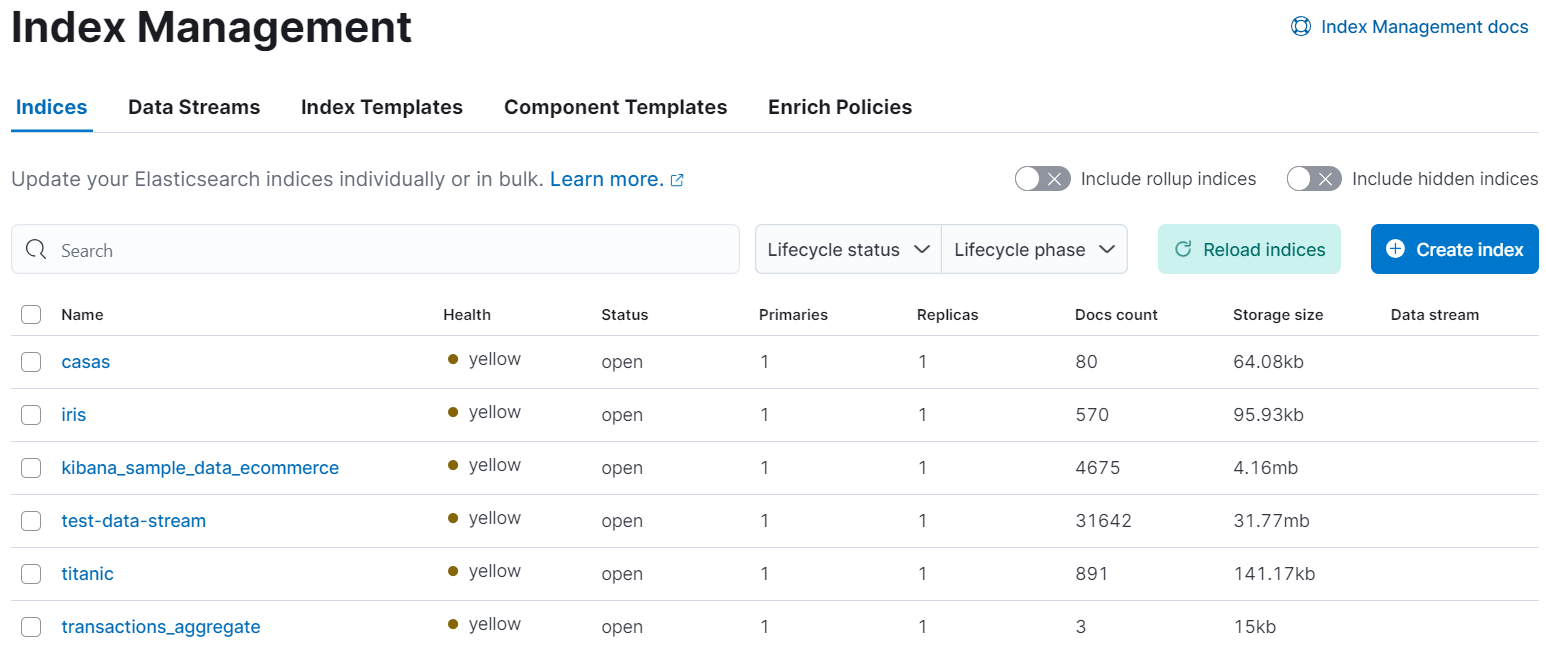
\includegraphics[width=1\linewidth]{img/management.png}
    \caption{Menú principal del \textit{Index Management} de Elastic.}
    \label{fig:indices}
\end{figure}

\section{Logstash}
Actuará como intermediador entre la fuente de datos y Elastic, es decir, cubrirá todo lo relacionado tanto con la parte de transformación de datos como con la de carga de los mismos. Cabe aclarar que se pueden cargar datos en Elastic sin Logstash, pero entonces se cargarían tal y como estén, por lo que todas las transformaciones necesarias tendrán que haberse hecho previamente. 

Permite definir \textit{pipelines} para procesar datos del lado de la fuente de ingesta de datos que permite transformarlos para después enviarlos y cargarlos en el destino indicado (i.e., ElasticSearch) \cite{Logstash}.

Logstash está enfocado tanto a la ingesta de datos, permitiendo cargar datos de múltiples orígenes con compatibilidad con protocolos, como al envío de datos a diversos destinos mediante un \textit{pipeline} configurable.

En este \textit{pipeline}, se pueden realizar modificaciones a los datos que entran. Algunos ejemplos de transformaciones con Logstash pueden ser estos:
\begin{itemize}
    \item El filtro \textit{mutate} permite cambiar nombres de campos, añadir nuevos o eliminar los que se consideren reduntantes. Un ejemplo de su uso es la figura \ref{fig:mutate} en la cuál se realiza un cambio de nombre de un campo, se añade un campo nuevo y se borra un campo.
    \item El filtro \textit{date} permite analizar campos que sean fechas indicándole con que formato están escritas. Un ejemplo de su uso es la figura\ref{fig:date}.
    \item El filtro \textit{csv} permite analizar los campos presentes en un fichero de tipo CSV de manera que divida cada línea en campos indicados. Un ejemplo de su uso es la figura\ref{fig:csv}.

\end{itemize}

\begin{figure}
    \centering
    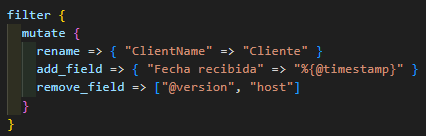
\includegraphics[width=1\linewidth]{img/mutate.png}
    \caption{Ejemplo de uso de filtro \textit{mutate}}
    \label{fig:mutate}
\end{figure}

\begin{figure}
    \centering
    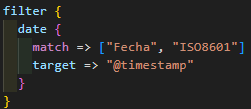
\includegraphics[width=1\linewidth]{img/date.png}
    \caption{Ejemplo de uso de filtro \textit{date}}
    \label{fig:date}
\end{figure}

\begin{figure}
    \centering
    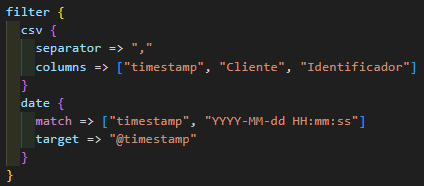
\includegraphics[width=1\linewidth]{img/csv.png}
    \caption{Ejemplo de uso de filtro \textit{csv}}
    \label{fig:csv}
\end{figure}

\paragraph{    }
\paragraph{  }
\paragraph{  }

\section{Kibana}
Por último, la parte de final del stack esta protagonizada por este programa, que se encargará de ejecutar las analíticas de los datos mandados por Logstash a Elastic y de mostrarlos en diferentes \textit{dashboards} con gráficas de datos que nos permitirá generar interacciones que resulten útiles e interesantes \cite{Kibana}.

Kibana permíte administrar los datos presentes en Elastic desde el apartado \textit{Data Views}. Facilita el acceso a los diferentes índices de datos de manera que genera un \textit{view} el cuál consiste en una representación de los datos de un índice para que puedan haber representaciones de los datos en un \textit{dashboard}. \ref{fig:dataviews}

Una vez se accede una \textit{view}, el apartado \textit{Discoverer} es la herramienta que facilita Kibana para poder ver de manera completa la información de los datos presentes en un índice. Se pueden aplicar filtros o clasificaciones para encontrar determinados datos. \ref{fig:discoverer}

Por útlimos, la función principal de Kibana es crear \textit{dashboards} con visualizaciones y demás herramientas sobre los datos presentes en Elatic a través del apartado \textit{Dashboards}, en el cuál se desarrollan tanto la creación como modificación de estos. \ref{fig:dashboard}.

\begin{figure}
    \centering
    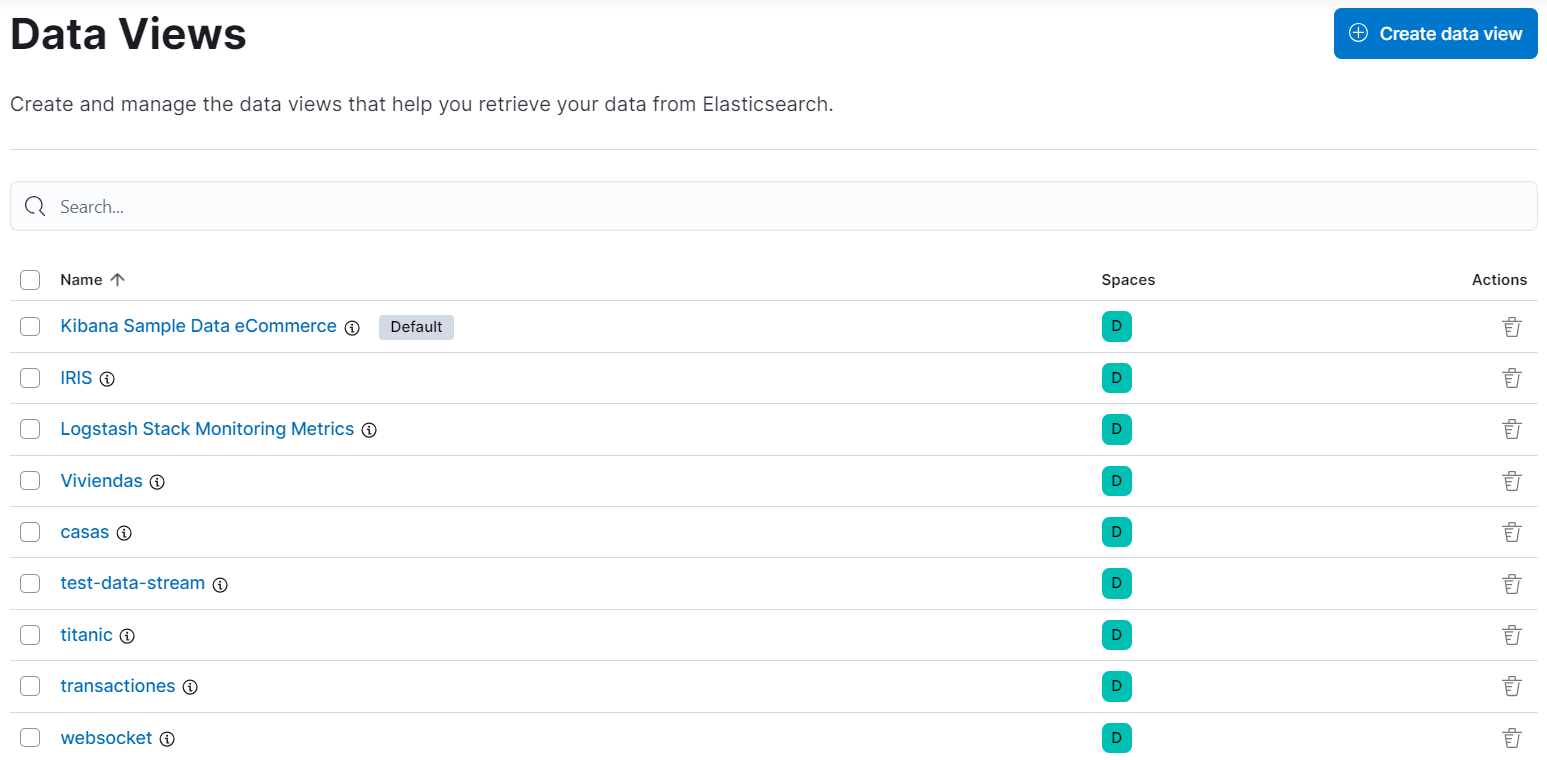
\includegraphics[width=1\linewidth]{img/views.png}
    \caption{Menú principal de los \textit{Data Views} de Kibana.}
    \label{fig:dataviews}
\end{figure}

\begin{figure}
    \centering
    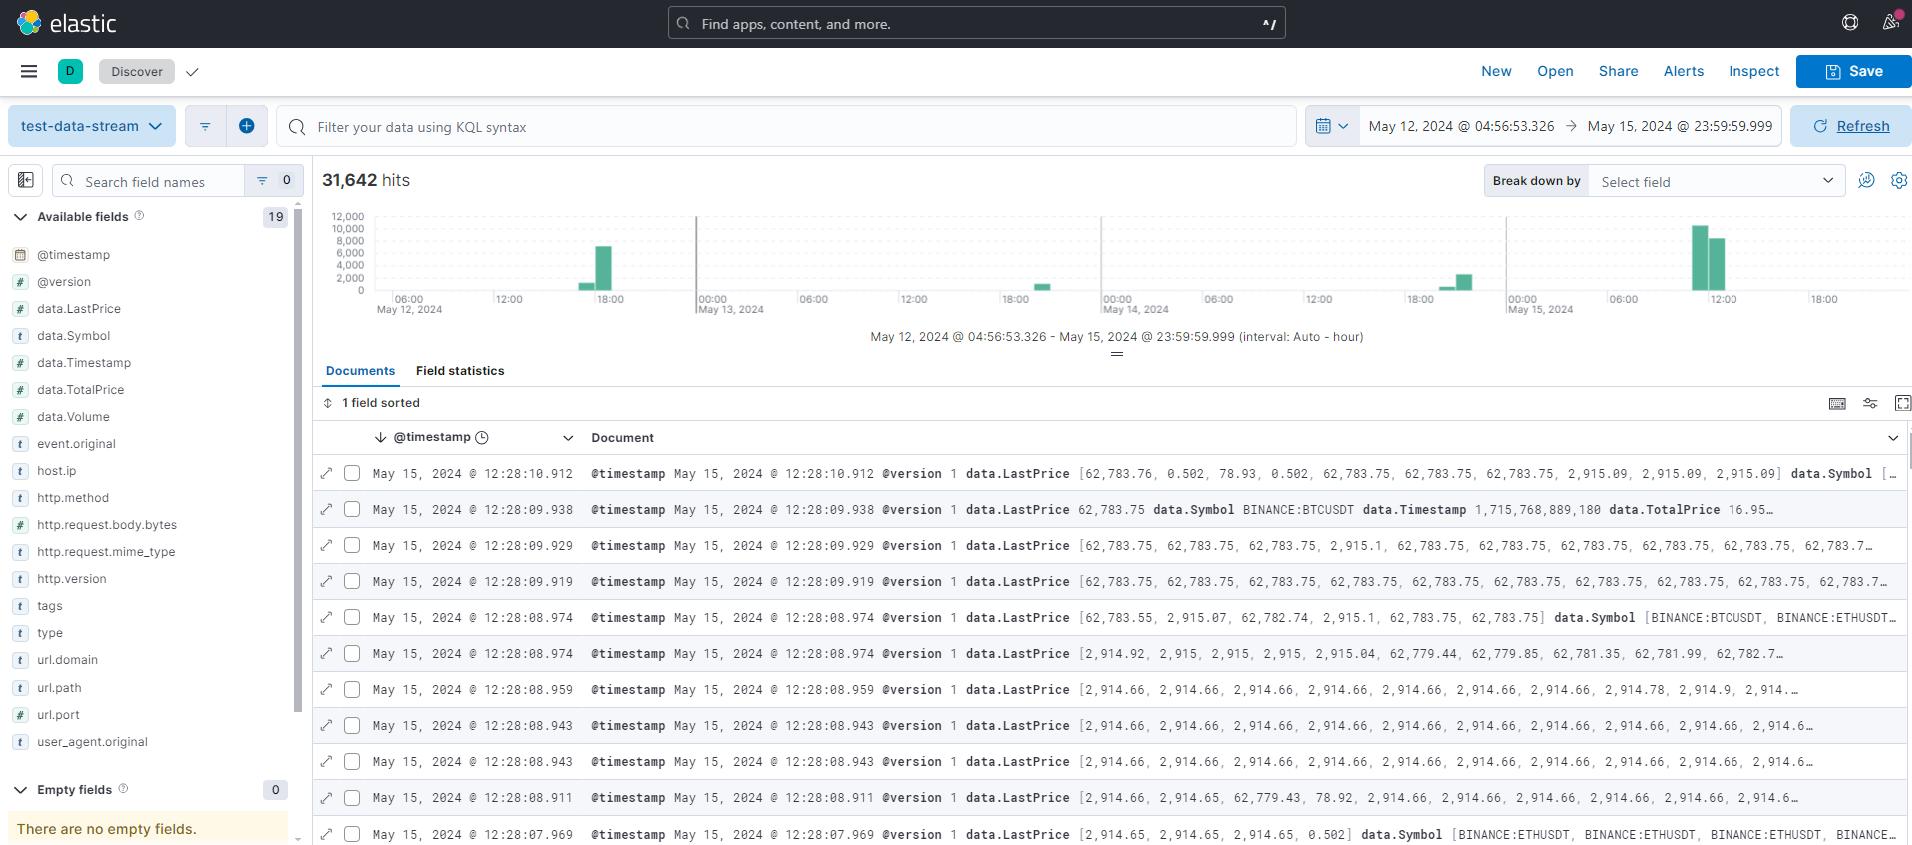
\includegraphics[width=1\linewidth]{img/discoverer.png}
    \caption{Apartado \textit{Discoverer}}
    \label{fig:discoverer}
\end{figure}

\begin{figure}
    \centering
    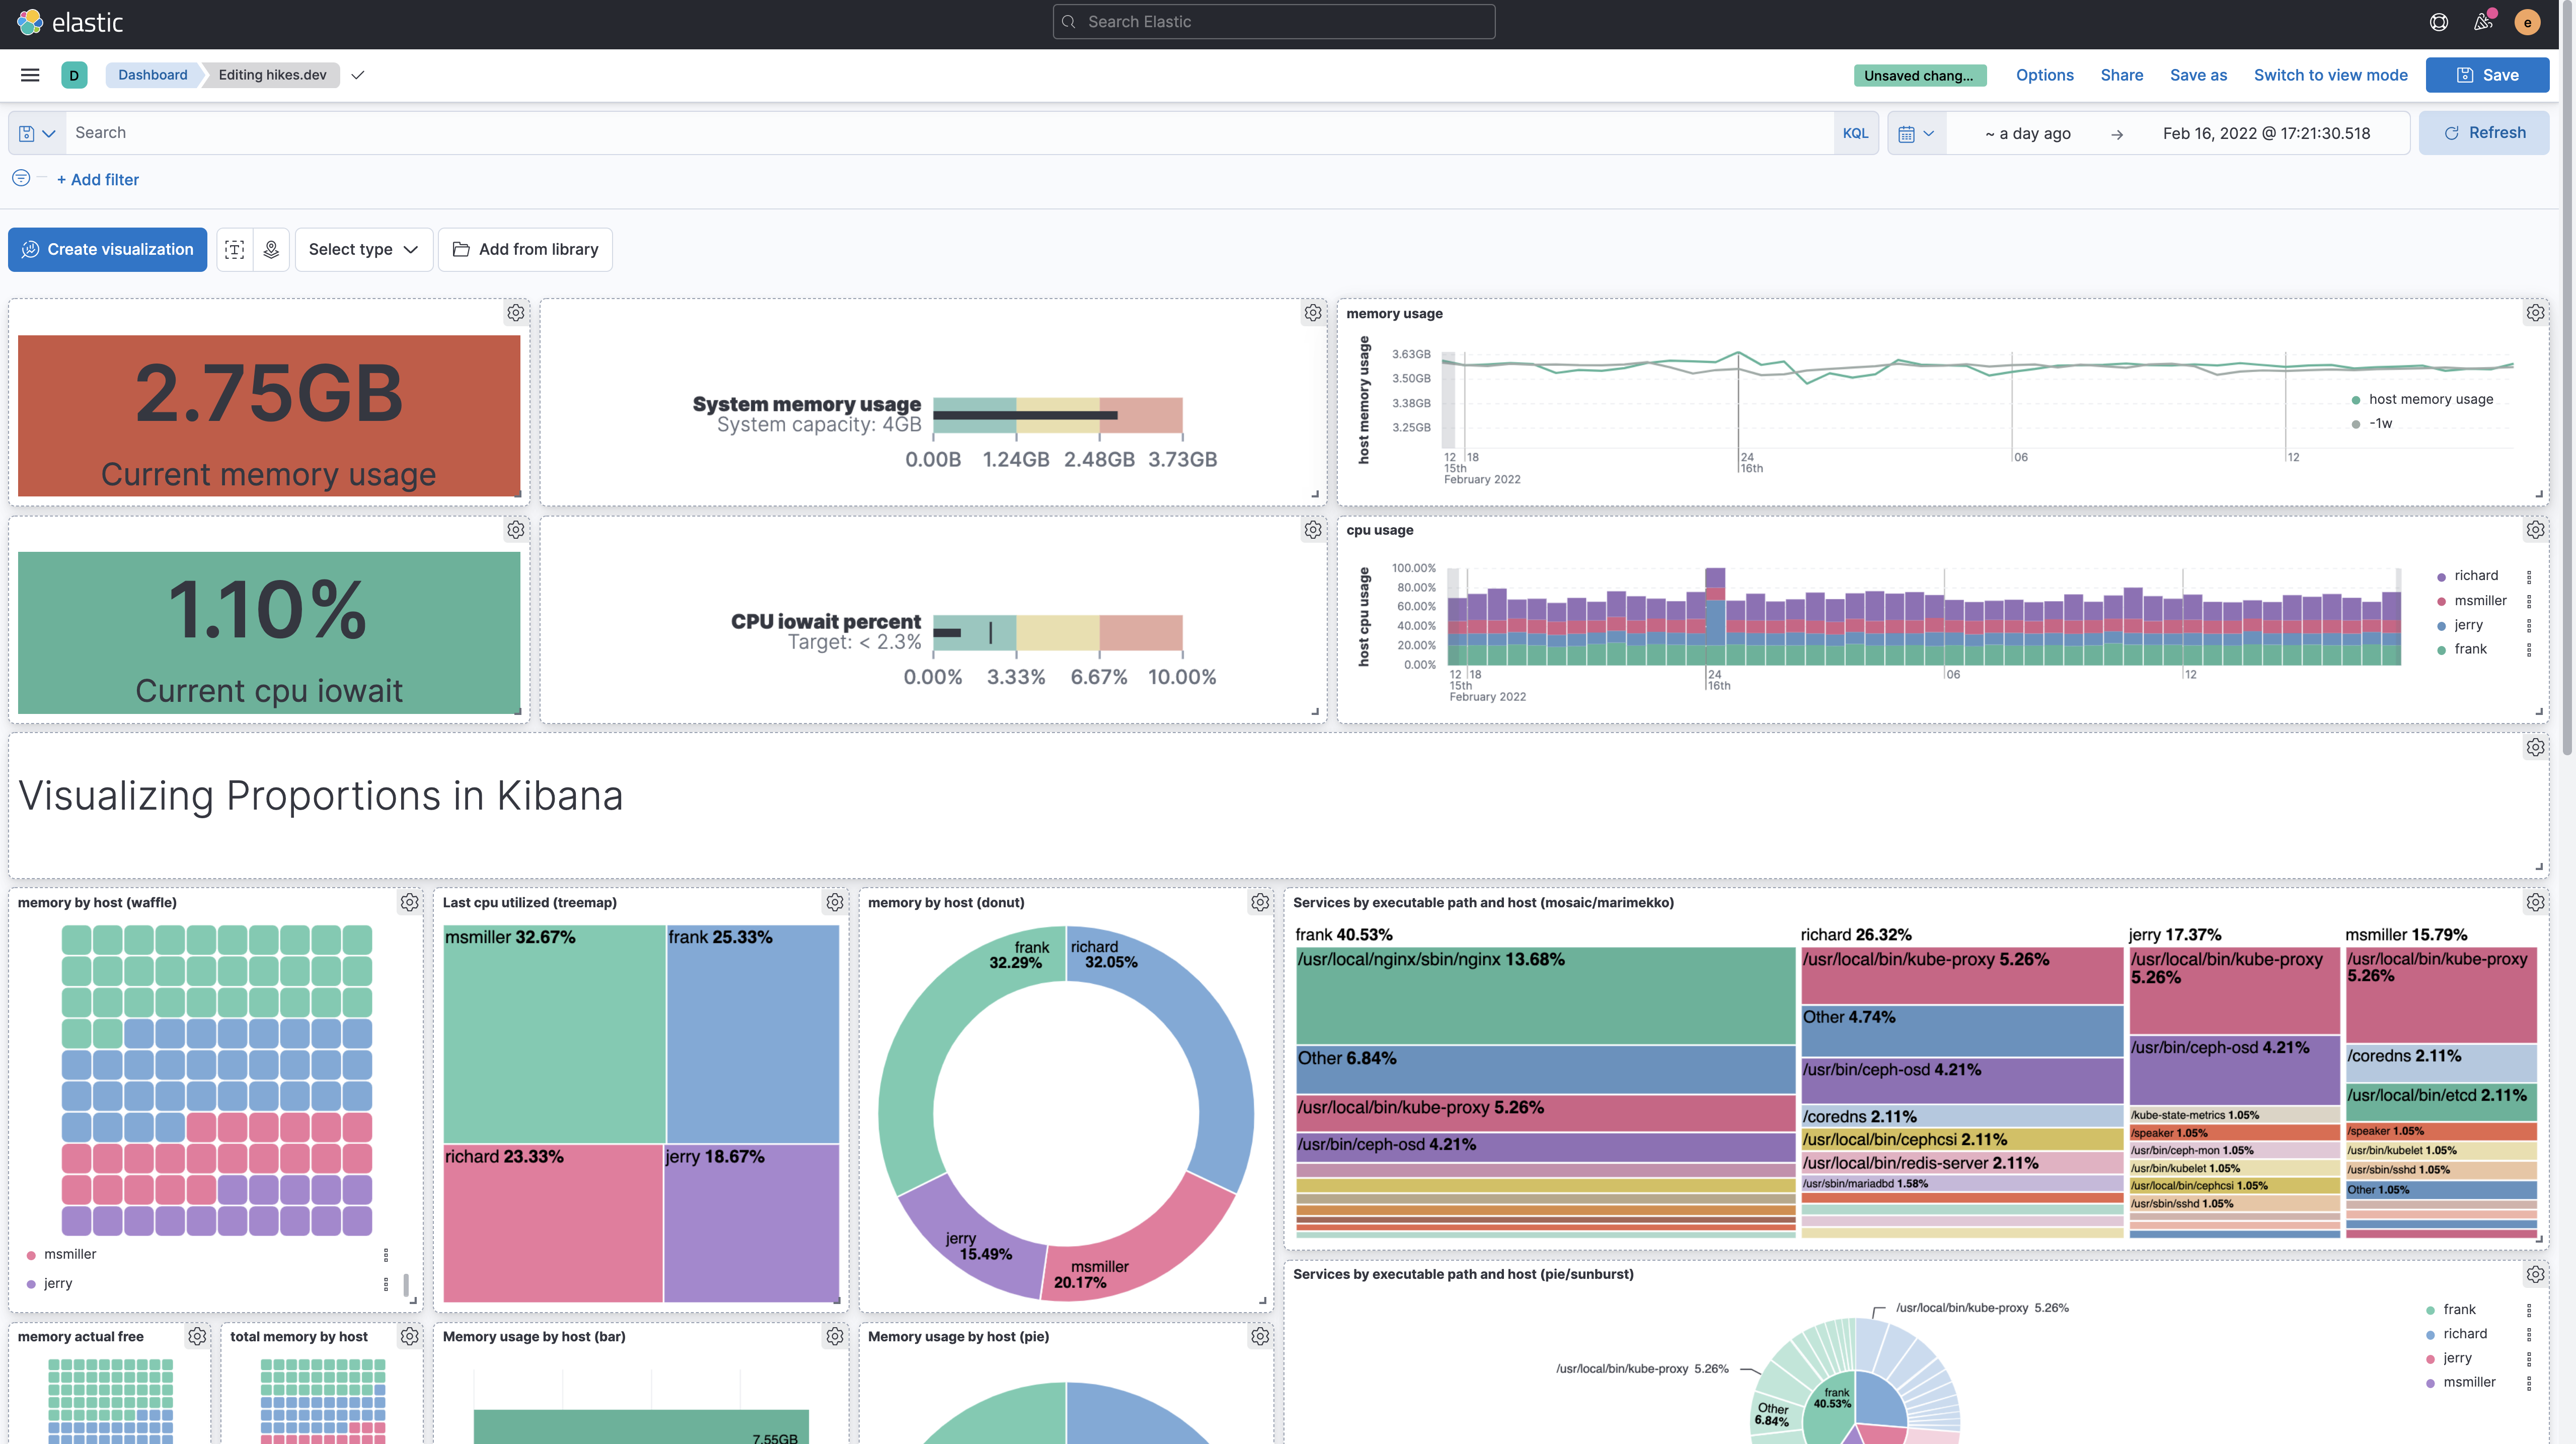
\includegraphics[width=1\linewidth]{img/kibana1.png}
    \caption{Dashboard de Kibana}
    \label{fig:dashboard}
\end{figure}

\section{Miscelánea}

\subsection{Scikit-Learn}
Biblioteca de aprendizaje automático de código abierto para \textit{Python} que permite utilizar algoritmos de clasificación, regresión, clustering y reducción de características a los datos que se le indiquen \cite{scikit}.

\subsection{Jupyter Notebook}
Aplicación web basada en \textit{Python} que se usará para crear y compartir documentos en los que realizamos cálculos computacionales con el resto del entorno de trabajo de los escenarios planteados \cite{jupyter}.

\subsection{Python}
Este lenguaje de programación permite el diseño e implementación de manera sencilla y eficiente de \textit{scripts}, en los cuales se emplean diferentes bibliotecas que utilizaremos para procesar los datos de diferentes maneras. Una vez finalizados son integrados en nuestro ecosistema de trabajo para ofrecer ayuda en distintos escenarios \cite{python}.

\subsection{Visual Studio Code}
Editor de código fuente desarrollado por Microsoft que permite crear, depurar y procesar archivos de código con total soltura. En este proyecto será empleado como apoyo para los diferentes \textit{scripts} de procesamiento de datos realizados \cite{code}.

\subsection{Overleaf}
Editor online de LATEX que permite la edición y exportación de documentos con este formato de manera fácil y rápida. En este proyecto tiene utilidad en la parte de la documentación tanto de la memoria como de los anexos \cite{overleaf}.

\subsection{GitHub}
Este \textit{software} sirve como alojamiento de proyectos, permitiendo modificaciones en el mismo, creaciones de archivos, modificaciones y demás. Será utilizado para mantener un orden en cuánto a la evolución del proyecto \cite{github}.